%
%%% REFERENCE
%
\section{教科書,参考文献}
%\begin{frame}
%\frametitle{教科書}
%  \begin{itemize}
%\item CS 第 1 とおなじ
%\item 教科書: 渡辺治 著,コンピュータサイエンス\textendash 計算を通して世界を観る, 丸善出版 (2015)
%\item 教科書のサイト: \href{http://www.is.titech.ac.jp/~watanabe/csbook/}{\beamerbutton{http://www.is.titech.ac.jp/$\sim$watanabe/csbook/}} 
%\item 4b(CS2) クラスのサイト: \href{https://sites.google.com/a/presystems.xyz/sample/home/elementary-computer-science}{\beamerbutton{https://sites.google.com/a/presystems.xyz/sample/home/elementary-computer-science}} 
%  \end{itemize}
%\centering
%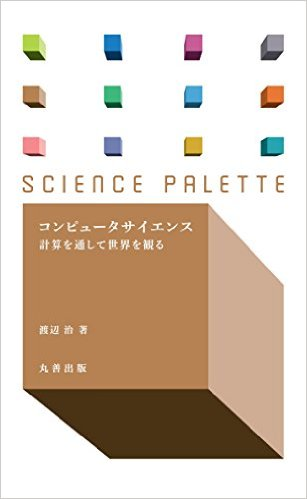
\includegraphics[scale=.25]{./Figure/TextBook.jpg}
%\end{frame}
\begin{frame}[shrink]
\frametitle{参考図書}
  \begin{itemize}
\item \href{https://www.mheducation.com/highered/product/discrete-mathematics-applications-rosen/M0073383090.html}{\beamerbutton{Discrete Mathematics and its Applications}}
\item Structure and Interpretation of Computer Programs \href{http://web.mit.edu/alexmv/6.037/sicp.pdf}{\beamerbutton{http://web.mit.edu/alexmv/6.037/sicp.pdf}} 
\item 計算機プログラムの構造と解釈 (日本語訳)\\ \href{http://sicp.iijlab.net/fulltext/xcont.html}{\beamerbutton{http://sicp.iijlab.net/fulltext/xcont.html}} 
  \end{itemize}
  \begin{columns}[c]
    \begin{column}{0.5\textwidth}
\centering
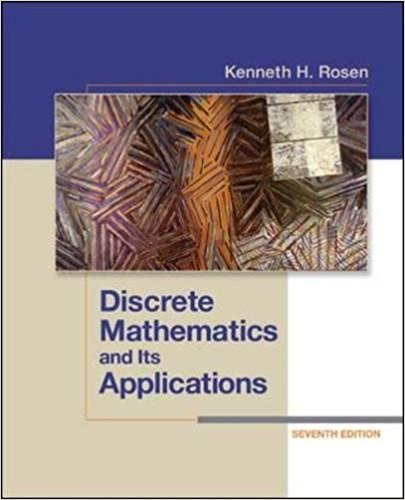
\includegraphics[scale=.25]{./Figure/Discrete_Mathematics_And_its_Applications.jpg}
    \end{column}
    \begin{column}{0.45\textwidth}
\centering
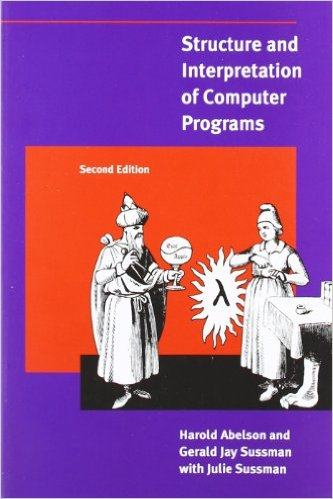
\includegraphics[scale=.25]{./Figure/SICP.jpg}
    \end{column}
  \end{columns}
\end{frame}
%
%%% GOAL
%
\section{講義概要}
\begin{frame}
\frametitle{講義概要}
  \begin{itemize}
\item この講義も Zoom で行います
\item 講義スケジュール:
    \begin{enumerate}
\item 再帰
\item よいアルゴリズム,わるいアルゴリズム,ふつうのアルゴリズム
%\item 大きい数と小さい数の計算 (実数の計算)
    \end{enumerate}
  \end{itemize}
  \begin{block}{目標}
計算でものを表すとき便利な道具と注意すべきことを会得すること
  \end{block}
\end{frame}
%
%%% EVALUATION
%
\section{評価基準}
\begin{frame}
\frametitle{評価基準}
  \begin{itemize}
\item 講義は全 7 回
\item 課題: 3 回 (計 85 点) と特別課題 (15 点)
\item 課題提出: 
    \begin{itemize}
\item 講義時間中に課題を出します
\item 提出方法はその都度指定します
    \end{itemize}
  \end{itemize}
\end{frame}
